\documentclass{article}

\usepackage[final]{style}
\usepackage[utf8]{inputenc} % allow utf-8 input
\usepackage[T1]{fontenc}    % use 8-bit T1 fonts
\usepackage{hyperref}       % hyperlinks
\usepackage{url}            % simple URL typesetting
\usepackage{booktabs}       % professional-quality tables
\usepackage{amsfonts}       % blackboard math symbols
\usepackage{nicefrac}       % compact symbols for 1/2, etc.
\usepackage{microtype}      % microtypography
\usepackage{verbatim}
\usepackage{graphicx}       % for figures
\usepackage{amsmath}


\title{Lecture Week-Recess: Optimal Control and Planning}

\author{
  Tan Ying Kiat, Vikash Ranjan \\
  \texttt{yingkiat(at)u.nus.edu, STUDENT2, etc.} \\
}

\begin{document}

\maketitle


\section{Model-Based Reinforcement Learning}
The objective of reinforcement learning is 
\begin{equation}
    \underbrace{\textit{p}_\theta(\textbf{s}_1,\textbf{a}_1,...,\textbf{s}_\textit{T},\textbf{a}_\textit{T})}
    _{\pi_\theta(\tau)} 
    = \textit{p}(\textbf{s}_1) \prod_{\textit{t}=1}^\textit{T}\pi_\theta(\textbf{a}_t\mid\textbf{s}_t)\textit{p}(\textbf{s}_{t+1}\mid\textbf{s}_t,\textbf{a}_t)
\end{equation}

\begin{equation}
    \theta^* = \arg\max_\theta \textit{\E}_{\tau\sim\textit{p}_\theta(\tau)}
    \bigg[\sum_{\textit{t}}\textit{r}(\textbf{s}_t,\textbf{a}_t)\bigg]
\end{equation}


\subsection{Recap of Model-Free Reinforcement Learning}
In model-free learning, we assume that the transition probability $\textit{p}(\textbf{s}_{t+1}\mid\textbf{s}_t,\textbf{a}_t)$
is unknown and we can bypass it by sampling. 

\subsection{What if we knew the transition dynamics?}
If we know the transition probability, it can make things easier because it becomes an optimisation problem.

And often we do know the transition dynamics, for example in games, easily modeled systems (such as navigating a car), and simulated environments (such as video games). We can learn the dynamics by system identification and learning.

This week's focus is on how to find out the action to take if we \textit{\textbf{know}} the transition probability.

\subsubsection{Deterministic}
For the deterministic case, we want to find the arg max.
\begin{equation}
    \textbf{a}_1,...,\textbf{a}_\textit{T} 
    = \arg\max_{\textbf{a}_1,...,\textbf{a}_\textit{T}}
    \sum_{\textit{t}=1}^\textit{T} \textit{r}(\textbf{s}_t,\textbf{a}_t)
    \; s.t. \; \textbf{a}_{t+1} = f(\textbf{s}_t,\textbf{a}_t)
\end{equation}

\subsubsection{Stochastic Open-Loop}
For the stochastic open-loop case, we should choose the best expectation, but this may be sub-optimal. As a corollary, if you buy lottery, you may not win even if it is the most optimal expectations.This is because taking action may not get you to an expected state.

\begin{equation}
    \textit{p}_\theta(\textbf{s}_1,...\textbf{s}_\textit{T} \mid \textbf{a}_1,...,\textbf{a}_\textit{T})
    = \textit{p}(\textbf{s}_1) \prod_{\textit{t}=1}^\textit{T}\textit{p}(\textbf{s}_{t+1}\mid\textbf{s}_t,\textbf{a}_t)
\end{equation}

\begin{equation}
    \textbf{a}_1,...,\textbf{a}_\textit{T} 
    = \arg\max_{\textbf{a}_1,...,\textbf{a}_\textit{T}} \textit{E} \bigg[\sum_{\textit{t}}\textit{r}(\textbf{s}_t,\textbf{a}_t) \mid \textbf{a}_1,...,\textbf{a}_\textit{T} \bigg]
\end{equation}


\subsubsection{Stochastic Closed-Loop}
For the stochastic closed-loop case, it can be considered as a special case of open-loop, where t=1. \textit{(Or is the open-loop a special case of the closed loop?)}

\begin{equation}
    \textit{p}(\textbf{s}_1,\textbf{a}_1,...\textbf{s}_\textit{T}, \textbf{a}_\textit{T})
    = \textit{p}(\textbf{s}_1) \prod_{\textit{t}=1}^\textit{T}
    \pi(\textbf{a}_\textit{t} \mid \textbf{s}_\textit{t} )
    \textit{p}(\textbf{s}_{t+1}\mid\textbf{s}_t,\textbf{a}_t)
\end{equation}

\begin{equation}
    \pi 
    = \arg\max_{\pi} \textit{E}_\textit{\E}_{\tau\sim\textit{p}(\tau)} \bigg[\sum_{\textit{t}}\textit{r}(\textbf{s}_t,\textbf{a}_t) \bigg]
\end{equation}

As an aside, on-policy/off-policy is a learning problem, while open-loop/closed-loop is a planning problem. They two (policy vs loop) are not correlated, although there are some similarities. Also of note, "global" optimises policy fo the entire existence of the problem, while "local" optimises for that particular timestep.

\section{Stochastic Optimization Methods}
\subsection{"Guess & Check" or "Random Shooting Method"}
We have to solve optimisation problem in equation (3). The easiest way is not to worry that there are sequence of events and treat it like any other optimisation problem. We can abstract away optimal control/planning:

\begin{equation}
    \textbf{a}_1,...,\textbf{a}_\textit{T} 
    = \arg\max_{\textbf{a}_1,...,\textbf{a}_\textit{T}}
    \underbrace{\textit{J}(\textbf{a}_1,...,\textbf{a}_\textit{T})}_{don't\; care\; what\; this\; is}
\end{equation}

\begin{equation}
    \textbf{A} = \arg\max_{\textbf{A}} \textit{J}(\textbf{A})
\end{equation}

The simplest method is the "guess and check" or "random shooting method":

\begin{enumerate}
    \item pick $\textbf{A}_1,...,\textbf{A}_\textit{N} $ from some distribution.
    \item choose $\textbf{A}_{i}$ based on $arg \; max_i \; \textit{J}(\textbf{A}_{i})$
\end{enumerate}

\subsection{Cross-Entropy Method (CEM)}
The Cross-Entropy Method (CEM) works for continuous-valued inputs:

\begin{enumerate}
    \item sample $\textbf{A}_1,...,\textbf{A}_\textit{N} $ from $\textit{p}(\textbf{A})$
    \item evaluate $\textit{J}(\textbf{A}_1),...,\textit{J}(\textbf{A}_N) $
    \item pick the \textit{elites} $\textbf{A}_{i1},...,\textbf{A}_\textit{iM} $ with highest value, where M < N
    \item refit $\textit{p}(\textbf{A})$ to the elites $\textbf{A}_{i1},...,\textbf{A}_\textit{iM} $
    \item go back to step (1)
\end{enumerate}

The intuition is that if it is around the "good value", then we will likely find the optimal solution near there. This method works better in continuous space but is also dependent on the distribution.

This method will converge towards a single action because the optimisation dimension is not too big. The termination criteria is when the rewards do not change much anymore. The convergence is when the probability changes are geting smaller and smaller over time ("hill climbing aspect") and not because of N shrinking. The convergence is likely towards local, and not global, optimisation.

Other things to note
\begin{itemize}
    \item Step 2 is parallelizable
    \item There is a "harsh dimensionality limit" because to cover the dimensions well, we may need an exponential number of samples to get some idea of the local landscape. However, this may not be practical.
    \item This method may also be used for closed-loop planning, but it could be very expensive.
\end{itemize}


\subsection{Monte Carlo Tree Search (MCTS)}
The Monte Carlo Tree Search algorithm is as follows:
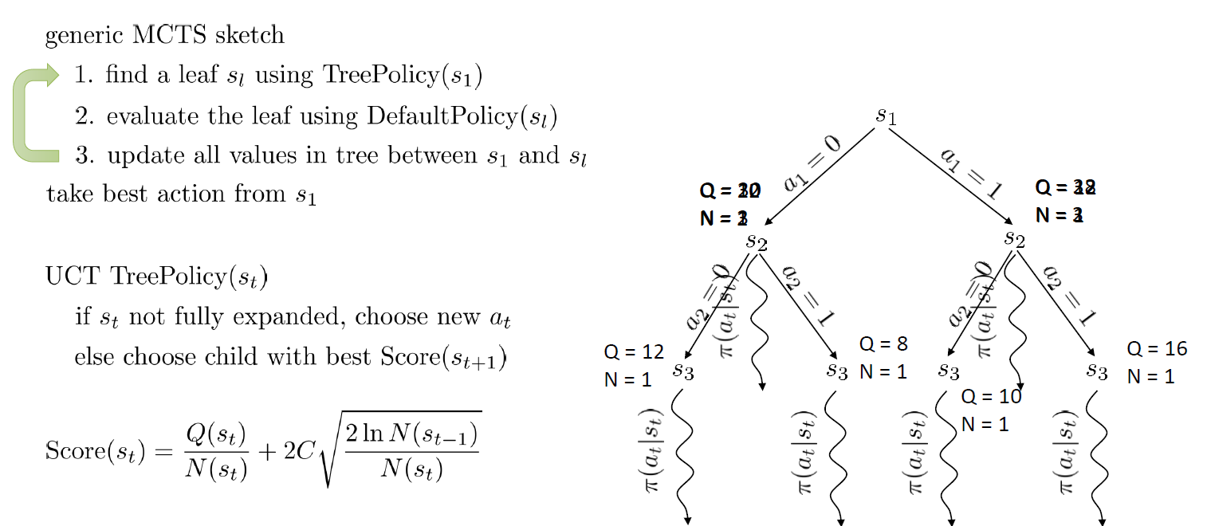
\includegraphics[scale=0.5]{MCTS.png}

\begin{itemize}
    \item The default policy is random sampling.
    
    \item Trying to balance between exploitation and exploration. C is the hyperparameter to tune this balance between exploitation and exploration.
    
    \item The score $s_t$ is used to pick a node for expansion based on the score and the rarity of the node having been visited.
    
    \item Typically, the algorithm will run 1 trajectory at a time, where the score is used to decide which child node to visit. Only upon the completion of the trajectory will it return to the first node.
    
\end{itemize}

\section{Trajectory Optimization: Linear Quadratic Regulation}
Optimal control is about operating a dynamic systems at minimum cost. Linear quadratic (LQ) problems are whee the system dynamics are represented by linear differential equations, and the cost (or rewards) is represented by a quadratic function. Hence Linear quadratic regulation (LQR) is used to solve LQ problems.

LQR can be used for a special case of a finite horizon.

Slides 29 to 35 from the presentation deck contains the LQR algorithm. Briefly, the summary of the algorithm is given here:
\begin{enumerate}
    \item (if necessary) estimate parameters $\textit{A}_t, \textit{B}_t,\Sigma_t$
    
    \item initialize $\Phi_T := -\textit{U}_T$ and $\Psi_T:=0$
    
    \item iterate from \textit{t} = \textit{T} - 1...0 to update $\Phi_t$ and $\Psi_t$ using $\Phi_{t+1}$ and $\Psi_{t+1}$ using the discrete Ricatti equations. If there exists a policy that drives the state towards zero, then convergence is guaranteed.
    
\end{enumerate}



% References
\small
\bibliographystyle{plain}
\bibliography{bibliography}

Presentation deck used by Lee Yong Ler, Teo Kok Keong, Lin Qian during presentation for CS6101 on 28 Feb 2019.

http://rail.eecs.berkeley.edu/deeprlcourse/static/slides/lec-10.pdf

http://cs229.stanford.edu/notes/cs229-notes12.pdf

http://cs229.stanford.edu/notes/cs229-notes13.pdf

http://rail.eecs.berkeley.edu/deeprlcourse/static/slides/lec-10.pdf

https://en.wikipedia.org/wiki/Linear\%E2\%80\%93quadratic\_regulator

\end{document}